\documentclass{beamer}
\usepackage{graphicx}
\usepackage{tikz}
\title[]{Mathematics behind Dobble}
\date{November 3, 2017}
\DeclareSymbolFont{extraup}{U}{zavm}{m}{n}
\DeclareMathSymbol{\varheart}{\mathalpha}{extraup}{86}
\begin{document}
\begin{frame}
	\titlepage
\end{frame}
  \begin{frame}
    \frametitle{Agenda}
    \begin{itemize}
  	\item Introduction to Dobble card game
  	\item Mathematics behind Dobble
     \end{itemize}
  \end{frame}
  
  \begin{frame}
    \frametitle{Dobble card game}
    \framesubtitle{The facts}
    \begin{itemize}
    	\item Card game for kids
	\item Consists of 55 cards
	\item Each card has 8 different symbols
	\item There are 57 symbols in total
    \end{itemize}
    \begin{picture}(0,0)
    	\put(220,-40){\includegraphics[width=3.5cm]{images/dobble}}
    \end{picture}
  \end{frame}
  
  \begin{frame}
  	\frametitle{Dobble card game}
	\framesubtitle{How does it work?}
	\begin{center}
	\includegraphics[width=9cm]{images/dobble_game}
	\end{center}
  \end{frame}
  
  \begin{frame}
    \frametitle{Dobble card game}
    \framesubtitle{Main condition}
    \begin{figure}
    	\vspace{-1cm}
    	\includegraphics[width=6cm]{images/dobble_unique}
    \end{figure}
    \centering
    Each pair of cards has \underline{exactly} one common symbol
  \end{frame}

  \begin{frame}
  	\frametitle{Main question}
	Given $q$ symbols on each card:
	\begin{itemize}
		\item How many symbols are needed in total?
		\item How many cards can be made in total?
		\item How can such a card set be constructed?
	\end{itemize}
  \end{frame}
  
  \begin{frame}
  	\frametitle{Example}
	Given $8$ symbols on each card: how many symbols are needed?
	\begin{itemize}
		\item 2 cards: $2\cdot 7 + 1 = 15$ symbols
			\begin{center}
			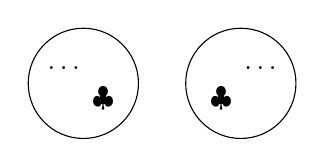
\begin{tikzpicture}
				\draw (2,2) circle (0.7cm);
				\node at (1.75,2.2) {$\dots$};
				\node at (2.25,1.8) {$\clubsuit$};
				\draw (4,2) circle (0.7cm);
				\node at (4.25,2.2) {$\dots$};
				\node at (3.75,1.8) {$\clubsuit$};
			\end{tikzpicture}
			\end{center}
		\item 3 cards: $3\cdot 6 + 3 = 21$ symbols
			\begin{center}
			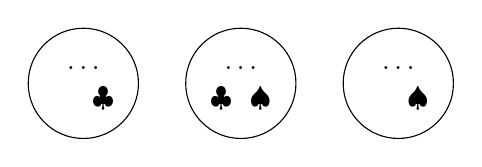
\begin{tikzpicture}
				\draw (2,2) circle (0.7cm);
				\node at (2,2.2) {$\dots$};
				\node at (2.25,1.8) {$\clubsuit$};
				\node at (1.75,1.8) {$\varheart$};
				\draw (4,2) circle (0.7cm);
				\node at (4,2.2) {$\dots$};
				\node at (3.75,1.8) {$\clubsuit$};
				\node at (4.25,1.8) {$\spadesuit$};
				\draw (6,2) circle (0.7cm);
				\node at (6,2.2) {$\dots$};
				\node at (5.75,1.8) {$\varheart$};
				\node at (6.25,1.8) {$\spadesuit$};
			\end{tikzpicture}
			\end{center}
	\end{itemize}
	\vspace{0.7cm}
	How to construct a large set of cards?
  \end{frame}
  
  \begin{frame}
  	\frametitle{Some mathematical background}
	\framesubtitle{A field}
	\begin{block}{Definition: field}
		A field is a set of elements, along with two functions defined on that set: 
		\begin{itemize}
			\item Addition function written as $a + b$
			\item Multiplication function written as $a \cdot b$
		\end{itemize}
		Each non-zero element of a field should have an inverse for the additional and multiplication.
	\end{block}
	\begin{exampleblock}{Examples}
		\begin{itemize}
			\item $\mathbb{Q}$, $\mathbb{R}$ and $\mathbb{C}$ are fields
			\item $\mathbb{Z}$ is not a field: no inverse for the multiplication
		\end{itemize}
	\end{exampleblock}
  \end{frame}
  \begin{frame}
  	\frametitle{Example: binary field}
	\framesubtitle{A field with two elements}
	\begin{itemize}
		\item A field should have at least two elements:
		\begin{itemize}
			\item Identity for the addition such that $a + 0 = a$
			\item Identity for the multiplication such that $a \cdot 1 = a$
		\end{itemize}
		\item The smallest field is a binary field with the following operations:

	\begin{center}
		\begin{tabular}{c | c c} 
 			$+$ & $0$ & $1$ \\ 
			\hline
 			$0$ & $0$ & $1$ \\ 
 			$1$ & $1$ & $0$
		\end{tabular}
		\qquad\qquad
		\begin{tabular}{c | c c} 
 			$\cdot$ & $0$ & $1$ \\ 
			\hline
 			$0$ & $0$ & $0$ \\ 
 			$1$ & $0$ & $1$
		\end{tabular}
	\end{center}
	This field is called $\mathbb{F}_2$.
		\end{itemize}
  \end{frame}
  \begin{frame}
  	\frametitle{Finite field}
	\begin{block}{Definition}
	Take $p$ a prime number, then $\mathbb{F}_p$ is a finite field, where
	\[
		\mathbb{F}_p = \mathbb{Z}/p\mathbb{Z} = \{\overline{0}, \overline{1}, \overline{2}, \dots, \overline{p-1} \}
	\]
	The addition and multiplication functions are defined by integer modulo operations. Note that $\overline{n} = n \mod p$.
	\end{block}
	\begin{exampleblock}{Examples}
		\begin{itemize}
			\item In $\mathbb{F}_{11}$: $\overline{7} + \overline{4} = \overline{11} = \overline{0}$
			\item In $\mathbb{F}_{13}$: The multiplication inverse of $\overline{8}$ is $\overline{5}$ because \[
			\overline{8} \cdot \overline{5} = \overline{8 \cdot 5} = \overline{40} = \overline{40 - 3\cdot13} =\overline{1}
		\]
			\item $\mathbb{F}_{12}$ is not a field because $\overline{3}\cdot\overline{4} = \overline{12} = \overline{0}$ while $\overline{3} \neq \overline{0}$ and $\overline{4} \neq \overline{0}$
		\end{itemize}
	\end{exampleblock}
  \end{frame}
  \begin{frame}
  	\frametitle{Little theorem of Fermat}
    \begin{picture}(0,0)
    	\put(225,-40){\includegraphics[width=3.5cm]{images/fermat}}
    \end{picture}	
    	\begin{block}{Little theorem of Fermat}
		If $p$ is a prime number, then for any integer $a$:\[
			a^p \equiv a \mod p
		\]
	\end{block}
	\begin{block}{Equivalent theorem}
		If $a$ is not divisible by $p$ then\[
			a^{p-1} \equiv 1 \mod p
		\]
	\end{block}
  \end{frame}
  \begin{frame}
  	\frametitle{Finite geometry}
	\framesubtitle{Geometry over a finite field $\mathbb{F}_p$}
	
	\begin{itemize}
		\item A geometric system that has only a finite number of points
		\item Example: finite affine plane of $\mathbb{F}_5$

	\begin{center}
	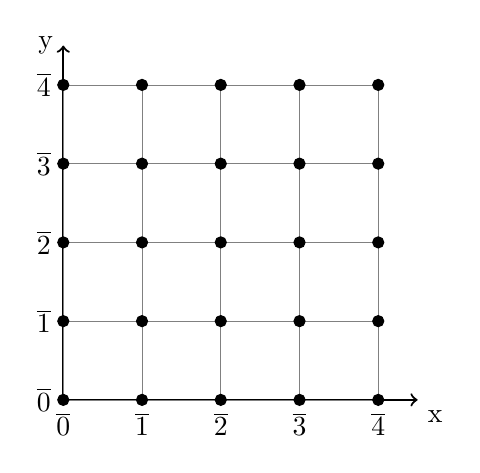
\begin{tikzpicture}
		\draw[thick,->] (0,0) -- (4.5,0) node[anchor=north west] {x};
		\draw[thick,->] (0,0) -- (0,4.5) node[anchor=east] {y};
		\foreach \x in {0,1,2,3,4}
    			{
			\draw (\x cm,1pt) -- (\x cm,-1pt) node[anchor=north] {$\overline{\x}$};
			 \draw (1pt,\x cm) -- (-1pt,\x cm) node[anchor=east] {$\overline{\x}$};
			}
		\draw[step=1cm,gray,very thin] (0,0) grid (4,4);
   		\foreach \x in {0,1,2,3,4}
		{
			\foreach \y in {0,1,2,3,4}
			{
				\filldraw [black] (\x,\y) circle (2pt);
			}
		}
	\end{tikzpicture}
	\end{center}
		\end{itemize}	
  \end{frame}
  \begin{frame}
  	\frametitle{Finite geometry}
	\framesubtitle{Lines in a finite affine field}
	Example in $\mathbb{F}_5$: $y = \overline{2}\cdot x + \overline{1}$
	\vspace{0.1cm}
	\begin{center}
		\begin{minipage}{0.40\textwidth}
		\begin{center}
		\begin{tabular}{c | c} 
 			$x$ & $y$ \\ 
			\hline
 			$\overline{0}$ & $\overline{1}$ \\ 
 			$\overline{1}$ & $\overline{3}$ \\ 
 			$\overline{2}$ & $\overline{0}$ \\
			$\overline{3}$ & $\overline{2}$ \\
			$\overline{4}$ & $\overline{4}$ \\
		\end{tabular}
		\end{center}
		\end{minipage}
		\begin{minipage}{0.58\textwidth}
	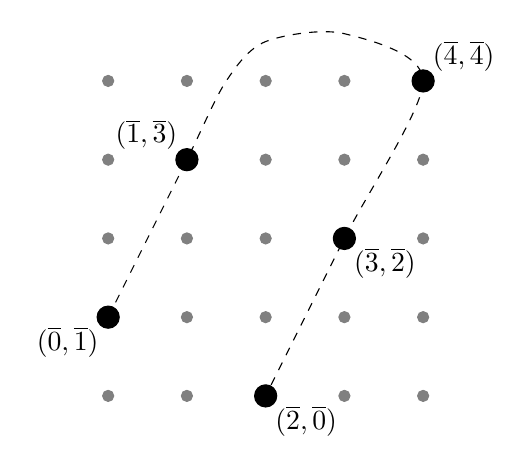
\begin{tikzpicture}
		\foreach \x in {0,1,2,3,4}
		{
			\foreach \y in {0,1,2,3,4}
			{
				\filldraw [gray] (\x,\y) circle (2pt);
			}
		}
		\draw [dashed] plot [smooth] coordinates {(0,1) (1,3) (1.5,4) (2,4.5) (3,4.6) (4,4) (3,2) (2, 0)};
		\filldraw [black] (0,1) circle (4pt) node[anchor=north east] {$(\overline{0},\overline{1})$};
		\filldraw [black] (1,3) circle (4pt) node[anchor=south east] {$(\overline{1},\overline{3})$};
		\filldraw [black] (2,0) circle (4pt) node[anchor=north west] {$(\overline{2},\overline{0})$};
		\filldraw [black] (3,2) circle (4pt) node[anchor=north west] {$(\overline{3},\overline{2})$};
		\filldraw [black] (4,4) circle (4pt) node[anchor=south west] {$(\overline{4},\overline{4})$};
		
	\end{tikzpicture}
	\end{minipage}
	\end{center}
  \end{frame}
  \begin{frame}
  	\frametitle{Dobble and geometry}
	\begin{block}{Geometry}
		Through any two points, there is exactly one line.
	\end{block}
	\begin{block}{Dobble}
		Two cards have exactly one common symbol.
	\end{block}
	\begin{center}
		\includegraphics[width=6cm]{images/dobble_line}
	\end{center}
  \end{frame}
  \begin{frame}
  	\frametitle{Dobble game with 4 symbols}
		A plane in $\mathbb{F}_2 = \{\overline{0}, \overline{1}\}$ consists of 
		\begin{itemize}
			\item 4 points: $(\overline{0},\overline{0})$, $(\overline{1},\overline{0})$, $(\overline{0},\overline{1})$ and $(\overline{1},\overline{1})$
			\item 6 lines:
			\begin{itemize}
				\item 2 vertical lines: $x = \overline{0}$ and $x = \overline{1}$
				\item 2 horizontal lines: $y = \overline{0}$ and $y = \overline{1}$
				\item 2 others: $y = x$ and $y = x + \overline{1}$
			\end{itemize}
		\end{itemize}
	\begin{center}
		\includegraphics[width=4cm]{images/dobble_4cards}
	\end{center}	
  \end{frame}
  \begin{frame}
  	\frametitle{Projective geometry}
	\begin{itemize}
		\item Not very pair of lines has an intersection point:
		\begin{center}
	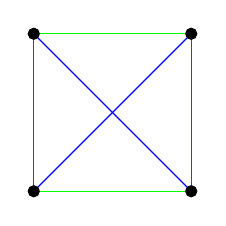
\begin{tikzpicture}
		\draw[red] (0,0) -- (0,2);
		\draw[red] (2,0) -- (2,2);
		\draw[green] (0,0) -- (2,0);
		\draw[green] (0,2) -- (2,2);
		\draw[blue] (0,0) -- (2,2);
		\draw[blue] (0,2) -- (2,0);
		\filldraw [black] (0,0) circle (2pt);
		\filldraw [black] (0,2) circle (2pt);
		\filldraw [black] (2,0) circle (2pt);
		\filldraw [black] (2,2) circle (2pt);
	\end{tikzpicture}
	\end{center}
	Parallel lines: 
	\begin{itemize}
		\item {\color{red}$x = \overline{0}$} and {\color{red}$x = \overline{1}$}
		\item {\color{green}$y = \overline{0}$} and {\color{green}$y = \overline{1}$}
		\item {\color{blue}$y = x$} and {\color{blue}$y = x + \overline{1}$}
	\end{itemize}
	\end{itemize}
  \end{frame}
  \begin{frame}
  	\frametitle{Projective geometry}
	\begin{itemize}
		\item Affine geometry is extended with points at infinity.
		\item Two \emph{parallel} lines intersect at infinity.
		\begin{center}
			\begin{tikzpicture}
				\node at (1,1.75) {$y = \overline{1}$};
				\node at (1,0.25) {$y = \overline{0}$};
				\node[gray] at (4.3,-0.4) {$\infty$};
				\draw [dashed] plot [smooth] coordinates {(0,0) (2,0) (3,0.25) (4,1)};
				\draw [dashed] plot [smooth] coordinates {(0,2) (2,2) (3,1.75) (4,1)};
				\draw[gray] (4,-0.5) -- (4,2.5);
				\filldraw [black] (0,0) circle (2pt);
				\filldraw [black] (0,2) circle (2pt);
				\filldraw [black] (2,0) circle (2pt);
				\filldraw [black] (2,2) circle (2pt);
				\filldraw [black] (4,1) circle (2pt);
			\end{tikzpicture}
		\end{center}
		\item There are no parallel lines in projective geometry
	\end{itemize}
  \end{frame}
  \begin{frame}
  	\frametitle{Projective geometry}
	\framesubtitle{Points}
	\begin{itemize}
		\item Euclidean plane: each point represented as a pair: $(x,y)$
		\item Projective plane: each point represented as a triple: $(x : y : z)$ where $x$, $y$ and $z$ are not all $0$.
		\begin{itemize}
		\item When $z \neq 0$, the point represented is the point $(x/z, y/z)$ in the Euclidean plane
		\item An Euclidean point $(x,y)$ maps to the projective point $(x : y : 1)$
		\item When $z = 0$, the point represented is a point at infinity
		\end{itemize}
		\item Note that $(x:y:z)$ and $(x/z : y/z : 1)$ represent the same point for $z \neq 0$
	\end{itemize}
  \end{frame}
  \begin{frame}
  	\frametitle{Projective geometry}
	\framesubtitle{Lines}
	\begin{itemize}
		\item A line is represented as follows \[
			ax + by + cz = 0
			\]
		\item For Euclidean geometry (where $z = 1$), this line corresponds with \[
			ax + by + c = 0
			\]
		\item The line $z = 0$ contains all points at infinity
	\end{itemize}
  \end{frame}
  \begin{frame}
  	\frametitle{Projective geometry}
	\framesubtitle{Duality}
	\begin{itemize}
		\item A point is represented by $(x:y:z) = (\alpha x : \alpha y : \alpha z)$ where $\alpha \neq 0$ and $x$,$y$,$z$ not all $0$.
		\item A line is represented by $[a : b : c] = [\alpha a : \alpha b : \alpha c]$ where $\alpha \neq 0$ and $a$,$b$,$c$ not all $0$.
	\end{itemize}
	\begin{block}{Duality principle}
		The role of points and lines are interchangeable
	\end{block}
	\begin{exampleblock}{Examples}
		\begin{itemize}
			\item Any two distinct points define a unique line.
			\item Any two distinct lines define a unique point.
		\end{itemize}
	\end{exampleblock}
  \end{frame}
  \begin{frame}
  	\frametitle{Back to Dobble}
	\begin{minipage}[t]{0.4\textwidth}
		\begin{center}
			\underline{Euclidean plane}\\
			\vspace*{2cm}
			\includegraphics[width=4cm]{images/dobble_4cards}
		\end{center}
	\end{minipage}
	\hspace*{1cm}
	\begin{minipage}[t]{0.48\textwidth}
		\begin{center}
			\underline{Projective plane}\\
			\vspace*{1cm}
			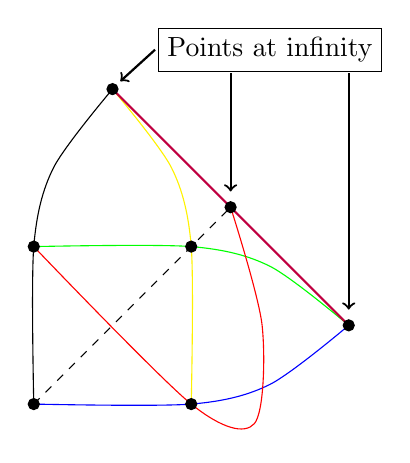
\begin{tikzpicture}
				\draw [blue] plot [smooth] coordinates {(0,0) (2,0) (3,0.25) (4,1)};
				\draw [green] plot [smooth] coordinates {(0,2) (2,2) (3,1.75) (4,1)};
				\draw [yellow] plot [smooth] coordinates {(2,0) (2,2) (1.75,3) (1,4)};
				\draw [black] plot [smooth] coordinates {(0,0) (0,2) (0.25,3) (1,4)};
				\draw [red] plot [smooth] coordinates {(0,2) (2,0) (2.8,-0.25) (2.9,1) (2.5,2.5)};
				\draw [dashed] (0,0) -- (2.5,2.5);
				\draw [purple, thick] (4,1) -- (1,4);
				\filldraw [black] (0,0) circle (2pt);
				\filldraw [black] (0,2) circle (2pt);
				\filldraw [black] (2,0) circle (2pt);
				\filldraw [black] (2,2) circle (2pt);
				\filldraw [black] (4,1) circle (2pt);
				\filldraw [black] (1,4) circle (2pt);
				\filldraw [black] (2.5,2.5) circle (2pt);
				\node [draw] at (3,4.5) {Points at infinity};
				\draw[thick,->] (1.54,4.5) -- (1.1,4.1);
				\draw[thick,->] (4,4.2) -- (4,1.2);
				\draw[thick,->] (2.5,4.2) -- (2.5,2.7);
			\end{tikzpicture}
		\end{center}
	\end{minipage}
  \end{frame}
  \begin{frame}
  	\frametitle{Back to Dobble}
	\framesubtitle{Another representation of the projective plane}
	\begin{minipage}[t]{0.48\textwidth}
		\begin{center}
			\underline{Projective plane}\\
			\vspace*{1cm}
			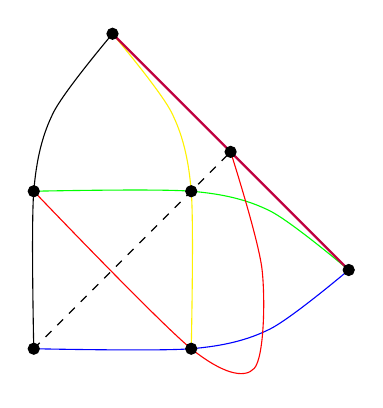
\begin{tikzpicture}
				\draw [blue] plot [smooth] coordinates {(0,0) (2,0) (3,0.25) (4,1)};
				\draw [green] plot [smooth] coordinates {(0,2) (2,2) (3,1.75) (4,1)};
				\draw [yellow] plot [smooth] coordinates {(2,0) (2,2) (1.75,3) (1,4)};
				\draw [black] plot [smooth] coordinates {(0,0) (0,2) (0.25,3) (1,4)};
				\draw [red] plot [smooth] coordinates {(0,2) (2,0) (2.8,-0.25) (2.9,1) (2.5,2.5)};
				\draw [dashed] (0,0) -- (2.5,2.5);
				\draw [purple, thick] (4,1) -- (1,4);
				\filldraw [black] (0,0) circle (2pt);
				\filldraw [black] (0,2) circle (2pt);
				\filldraw [black] (2,0) circle (2pt);
				\filldraw [black] (2,2) circle (2pt);
				\filldraw [black] (4,1) circle (2pt);
				\filldraw [black] (1,4) circle (2pt);
				\filldraw [black] (2.5,2.5) circle (2pt);
			\end{tikzpicture}
		\end{center}
	\end{minipage}
	\begin{minipage}[t]{0.48\textwidth}
		\begin{center}
		\underline{Fano representation}\\
		\vspace*{1cm}
		\includegraphics[width=5cm]{images/dobble_fano}
		\end{center}
	\end{minipage}		
  \end{frame}
  \begin{frame}
  	\frametitle{Summary of our mini Dobble}
	\begin{itemize}
		\item The finite field $\mathbb{F}_2$ of two elements is used
		\item Each card consists of 3 symbols
		\item There are 7 symbols in total
		\item There are 7 cards in total
	\end{itemize}
    \begin{picture}(0,0)
    	\put(180,-50){\includegraphics[width=5cm]{images/dobble_fano}}
    \end{picture}
  \end{frame}
  \begin{frame}
  	\frametitle{Dobble}
	\framesubtitle{Number of symbols}
	\begin{itemize}
		\item The number of symbols on a card it determined by \\
		the number of lines intersecting a single point
		\item In $\mathbb{F}_p$, there are $p+1$ lines going through a each point
		\item In $\mathbb{F}_p$, there are $p^2 + p + 1$ lines in total
		\begin{itemize}
			\item $y = ax + b$  \hspace{0.2cm} $p\cdot p$ lines 
			\item $x = a$ \hspace{1.15cm}$p$ lines
			\item $1$ line at infinity
		\end{itemize}
	\end{itemize}
  \end{frame}
   \begin{frame}
  	\frametitle{The real Dobble}
	\begin{itemize}
		\item The real Dobble has $7 + 1 = 8$ symbols on each card
		\item Therefore it is constructed using field $\mathbb{F}_7$
		\item In $\mathbb{F}_7$, there are $7^2 + 7 + 1 = 57$ lines.\\
		Therefore, there are $57$ symbols in Dobble
		\item Due to the duality, there are also $57$ cards. \\
		But in the actual game, there are only $55$ cards.
	\end{itemize}
  \end{frame}
  \begin{frame}
  	\frametitle{Summary}
	\begin{itemize}
		\item A card set can be constructed using projective geometry over a finite field $\mathbb{F}_p$
		\item There are as many cards as symbols due to the duality
		\item In the real Dobble, two cards are missing (55 vs 57)
	\end{itemize}
	\vspace{0.5cm}
	\begin{center}
	\includegraphics[width=6cm]{images/dobble_cards}
	\end{center}  	
  \end{frame}
   \begin{frame}
  	\frametitle{Dobble game}
	\framesubtitle{Is this a complete set?}
	\begin{itemize}
		\item Assume each card has $q$ symbols
		\item There are $m$ symbols in total: $S = \left\{ s_1, s_2, \dots, s_m\right\}$
		\item Take a fixed symbol $s$ and assume there are $k$ cards containing $s$
		\item Take another card which does not contain $s$, it should have a different symbol with every card
		\begin{center}
			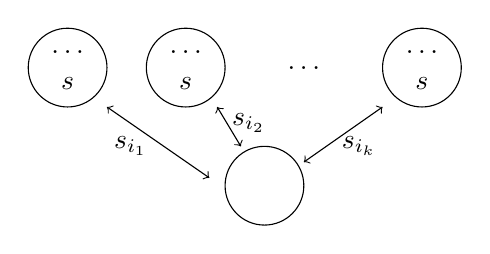
\begin{tikzpicture}
				\draw (2,2) circle (0.5cm);
				\node at (2,2.2) {$\dots$};
				\node at (2,1.8) {$s$};
				\draw (3.5,2) circle (0.5cm);
				\node at (3.5,2.2) {$\dots$};
				\node at (3.5,1.8) {$s$};
				\node at (5,2) {$\dots$};
				\draw (6.5,2) circle (0.5cm);
				\node at (6.5,2.2) {$\dots$};
				\node at (6.5,1.8) {$s$};
				\draw[<->] (2.5,1.5) -- (3.8,0.6);
				\node at (2.8,1) {$s_{i_1}$};
				\draw[<->] (3.9,1.5) -- (4.2,1);
				\node at (4.3,1.3) {$s_{i_2}$};
				\draw[<->] (6,1.5) -- (5,0.8);
				\node at (5.7,1) {$s_{i_k}$};
				\draw (4.5,0.5) circle (0.5cm);
			\end{tikzpicture}
		\end{center}
		\item All $s_{i_j}$ are different because otherwise a card will have at least two symbols in common. Therefore $k \leq q$
		\end{itemize}
  \end{frame}
  \begin{frame}
  	\frametitle{Dobble game}
	\framesubtitle{Is this a complete set?}
	\begin{itemize}
		\item Take a fixed card with symbols $\left\{s_{i_1},\dots,s_{i_q}\right\}$
		\item Assume there are
			\begin{itemize}
				\item $k_1 - 1$ other cards with symbol $s_{i_1}$
				\item $\dots$
				\item $k_q - 1$ other cards with symbol $s_{i_q}$
			\end{itemize}
		\item Since every card should have one symbol in common with the initial card. Therefore it is a full set. \[
		\sum_{j = 1}^q \left(k_j - 1\right) = n - 1
	\]
		\item Using $k \leq$ q: $n \leq q\left(q - 1\right) + 1$
		\item For the real Dobble: $n \leq 57$ since $q = 8$
	\end{itemize}
  \end{frame}
  \begin{frame}
  	\frametitle{References}
	\begin{enumerate}
		\item Dobble et La Geometrie Finie - Maxime Bourrigan \\
		{\scriptsize\url{http://images.math.cnrs.fr/Dobble-et-la-geometrie-finie.html}}
	\end{enumerate}
  \end{frame}
% etc
\end{document}